
To learn a policy for optimal landing an \textit{environment} is needed in the form of a rocket model. As this study provides aims to provide a benchmark for determining the feasibility of using policy learning to provide control to a rocket during landing, and no proprietary model is available, a new model is constructed based of physics and literature. First, to ensure a feasible landing the rocket is sized and staged through reviewing a case study rocket from industry in \autoref{sec:SpaceX} and then a paper which optimal stages a reusable rocket in \autoref{sec:OptimalStaging}. Following this an aerodynamic model is derived with parameters found from literature in \autoref{sec:Aerodynamics}, before the same with the grid fins acting as the manoeuvrable aerodynamic control surfaces in \autoref{sec:ACS}. Following this, the atmosphere and thruster models are found and derived in \autoref{sec:Atmosphere} and \autoref{sec:RocketEngines} respectively. Finally, the model is culminated into its equations of motion in \autoref{sec:EoM}.


\subsection{Starship case study}
\label{sec:SpaceX}

To ensure the rocket has the ability to land, it must be sized to be feasible. Currently their are only a handful of proven rockets with the ability to vertically takeoff and land, these are from \textit{Space X} and \textit{Blue Origin}. To size reasonable parameters for the rocket, the \textit{Starship} launch vehicle from Space X shall be reviewed, this is a two stage launcher with the first stage called the \textit{Super Heavy Booster}, and a second stage called its namesake \textit{Starship}. The mass of each stage is shown in \autoref{tab:starship_parameters}, with their structural coefficients calculated through \autoref{eq:structural_coeff}. This launcher is able to carry 100-150 tonnes to LEO orbit, and 27 to GEO orbit (\cite{SpaceX2020_StarshipGuide}).

\begin{equation}
    \epsilon = \frac{m_s}{m_s + m_p}
\label{eq:structural_coeff}
\end{equation}

\begin{table}[htbp]
    \centering
    \caption{Mass and performance parameters of \textit{Super Heavy} and \textit{Starship}}
    \label{tab:starship_parameters}
    \begin{tabular}{@{}lcc@{}}
        \toprule
        & \textbf{Super Heavy booster} & \textbf{Starship} \\ \midrule
        Total mass [t]                          & 3,675 & 1,600 (excluding payload) \\
        Propellant mass [t]                     & 3,400 & 1,500 \\
        Structural mass [t]  & 275    & 100 \\
        Structural coefficient [-] & 0.0748 & 0.0625 \\ \bottomrule
    \end{tabular}
\end{table}

In terms of propellant, both stages use a fuel oxidiser mixture of liquid oxygen ($LOX$) and liquid methane ($LCH_4$) called methalox. The 2nd stage carries 1170 kg of $LOX$ and 330 kg $LCH_4$, giving a oxidiser-fuel ratio of 3.545; this is taken to be the same for the first stage too due to the same engines, Raptor 3, being used.


The Raptor 3 engines are top of the range full-flow cycle engines, with two varieties. One optimised for sea-level performance which is used on the 1st stage. The second is optimised for vacuum performance, with the 2nd stage taking 3 of these for ascent and 3 sea-level optimised engines for descent. From the specific impulse, a measure of rocket efficiency giving the thrust produced per unit flow of propellant, the exhaust velocities are calculated through \autoref{eq:exhaust_velocities}. As the engines are optimised for sea-level and vacuum, the nozzle exit pressures are assumed to be close to the pressure in those regimes to minimise the pressure losses, \autoref{eq:pressure_losses}. The parameters of the Raptor 3 engine variants are displayed in \autoref{tab:raptor3}.

\begin{equation}
    v_{ex} = I_{sp} \cdot g_0
\label{eq:exhaust_velocities}
\end{equation}

\begin{equation}
    T_{\text{pressure losses}} = (p_e - p_a) \cdot A_e
\label{eq:pressure_losses}
\end{equation}

\begin{table}[h!]
    \centering
    \caption{Parameters of the Raptor 3 engines}
    \label{tab:raptor3}
    \begin{tabular}{@{}lcc@{}}
        \toprule
        & \textbf{Sea-level Raptor 3 } & \textbf{Vacuum Raptor 3} \\ \midrule
        Specific impulse [s] & 350 & 380 \\
        Exit diameter [m] & 1.3 & 1.3 \\
        Exit area [$m^2$] & 1.327 & 2.3 \\
        Thrust [$MN$] & 2.745 & 2 \\
        Engine mass (integrated) [kg] & 1525 (1720) & 1525 (1720) \\
        Exhaust velocities [$m/s$] & 3433.5 & 3727.8 \\
        Exit pressure estimate [$kPa$] & 101 & 0 \\
        Engine Height [$m$] & 3.1 & 4.6 \\
        \bottomrule
    \end{tabular}
\end{table}


The thrust-to-weight ratio ($TWR$) is a crucial parameter affecting how much acceleration the rocket can produce, especially at take-off. The engines produce a certain thrust, resulting in the $TWR$ determining how many engines are on the rocket. The $TWR$ is calculated through \autoref{eq:TWR} to give the stage's $TWR$ in \autoref{tab:TWR}.

\begin{equation}
    TWR = \frac{T^e_i \cdot n^e_i}{m_i \cdot g_0}
\label{eq:TWR}
\end{equation}

\begin{table}[h!]
    \centering
    \caption{Stage's thrust-to-weight ratio.}
    \label{tab:TWR}
    \begin{tabular}{@{}lcc@{}}
        \toprule
        & \textbf{Super Heavy booster} & \textbf{Starship} \\ \midrule
        Number of engines [-] & 33 & 6 \\
        Stage Thrust-to-Weight ratio [-] & 2.51 & 0.7645 \\
        \bottomrule
    \end{tabular}
\end{table}

Space X's $TWR$ can be used to decide the number of engines on a different sized rockets. The TWR for each stage can be used to calculate the stage's maximum thrust, mass flow and number of engines from its initial mass by \autoref{eq:n_e}.


\begin{equation}
\begin{aligned}
    T^{req}_i =&  m_i(0) \cdot g_0 \cdot TWR_i\\
    n^e_i =& [\frac{T^{req}_i}{T^{engine}_i}] \\
    T^{max}_i =& n^e_i \cdot T^{engine}_i \\
    \dot{m}_i^{max} =& \frac{T^{max}_i}{v_{ex}^i}
\end{aligned}
\label{eq:n_e}
\end{equation}



%Resultingrocketwidthandgiballledetccc
\subsubsection{Number of engines}
The number of engines is used to size the width of the rocket, such that the rocket can fit the required number of engines. \autoref{fig:Raptor_Comparison} shows the layout of the Raptor engines for the Super Heavy Booster, they layour with 20 fixed engines in the outer ring, followed by an inner ring of 10 gimballed engines and a central triangle of gimballed engines, totalling in 20 fixed engines and 13 gimballed engines. Taking the three centrally gimballed engines as fixed independent of the rocket's configuration, the number of engines within the ring are altered, knowing that 2 extra outer ring engines are needed to fit one extra gimballed engines.

\begin{equation}
    r_r = r_{\text{superheavy}} \cdot (1 + \frac{n_{\text{outer}} - n_{\text{outer,superheavy}}}{n_{\text{outer,superheavy}}})
\end{equation}

\begin{figure}[H]
    \centering
    \begin{subcaptionbox}{Raptor 3 engine\footnotemark[1]\label{fig:Raptor_3}}[0.35\linewidth]
        {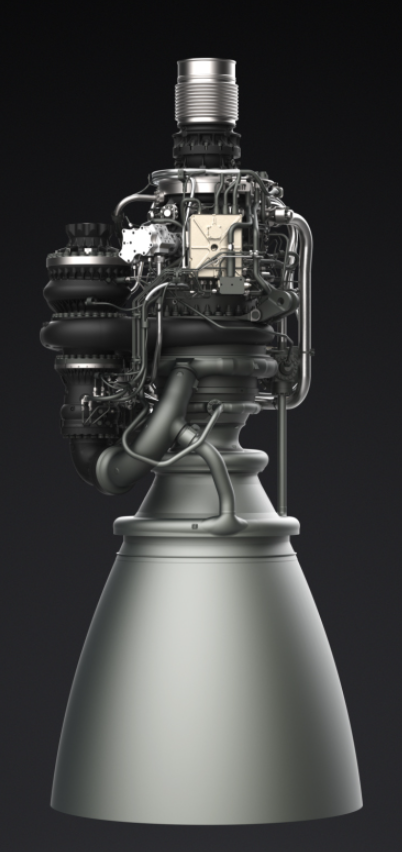
\includegraphics[width=\linewidth]{figures/LiteratureStudy/raptor_3.png}}
    \end{subcaptionbox}
    \hfill
    \begin{subcaptionbox}{Super Heavy engines\footnotemark[2]\label{fig:SuperHeavyEngines}}[0.58\linewidth]
        {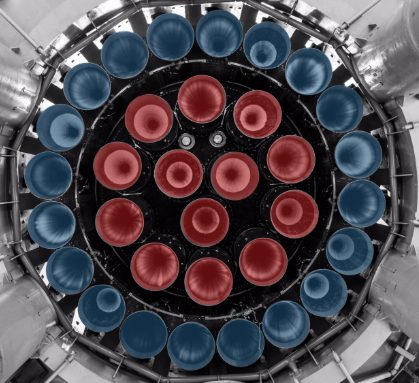
\includegraphics[width=\linewidth]{figures/LiteratureStudy/SuperHeavyRaptorLayour.png}}
    \end{subcaptionbox}
    \caption{Raptor 3 and Super Heavy engine layout}
    \label{fig:Raptor_Comparison}
    \footnotetext[1]{\url{https://www.spacex.com/vehicles/starship/}}
    \footnotetext[2]{\url{https://everydayastronaut.com/spacex-raptor-engine-comparison/}}
\end{figure}

\subsection{Optimal staging of a reusable rocket}
\label{sec:OptimalStaging}
As said in the previous section, a rocket must be sized such that it is feasible to land. If the Space X size was to be used it may not be feasible within in our model due to lower fidelity aerodynamics, or incorrect reporting of values from Space X. This results in a rocket needing to be independently sized. The method of \cite{ReusbaleStaging} is followed to size a two stage rocket with an reusable first stage and an expendable second stage.

First \autoref{eq:descent_eps} uses the first stage's structural coefficient for descent to calculate the velocity increment to descend. The structural coefficient for first stage descent is unknown, but can be the paper's value can be used. Later, this parameter can be updated from a trajectory optimiser results.

\begin{equation}
    \Delta v_{d,1} = v_{ex,1} \cdot \ln(\frac{1}{\epsilon_{d,1}}) \rightarrow \epsilon_{d,1} = e^{-\frac{\Delta v_{d,1}}{v_{ex,1}}}
\label{eq:descent_eps}
\end{equation}

The optimal staging procedure, as like expendable rockets, sets a parameter (here $\kappa$) in the X of the Tsiolkovsky equation, for \cite{ReusbaleStaging} this becomes \autoref{eq:Lagrangian_Tsiolkovsky}. When this equation is solved for $\kappa$ then the payload ratio shall be minimised, in turn minimising take off mass. The velocity increment required is found from the desired semi-major axis, \autoref{eq:v_req}.

The optimal staging procedure is similar to that of an expendable rocket. It starts by introducing a Lagrange multiplier $\kappa$ to perform constrained optimisation of the Tsiolkovsky rocket equation. This yields \autoref{eq:Lagrangian_Tsiolkovsky}, which when solved produces $\kappa$ to maximise the payload ratio; the fraction of the rocket's take-off mass consisting of payload. To do this the velocity increment required is set from the orbital velocity at the defined semi-major axis, as shown in \autoref{eq:v_req}.

To ensure feasibility of the Lagrange multiplier $\kappa$ the following constraints are added to ensure physical and mathematical validity:

\begin{itemize}
    \item \textbf{Exhaust velocity bound:} ensures $\kappa$ avoids singularities in the logarithmic expression.
    \[
    0 < \kappa < \min(v_{ex,1}, v_{ex,2})
    \]
    \item \textbf{Logarithm argument positivity:} guarantees that the logarithm's values are strictly positive to prevent undefined values.
    \[
    \frac{v_{ex,i} - \kappa}{v_{ex,i} \cdot \epsilon_i} > 0 \quad \Rightarrow \quad \kappa < v_{ex,i}
    \]
\end{itemize}


\begin{equation}
\begin{aligned}
    a =& y_t + R_E \\
    \Delta v_{req} =& \sqrt{\frac{\mu}{a}}
\end{aligned}
\label{eq:v_req}
\end{equation}

\begin{equation}
    \Delta v_{req} = v_{ex,1} \cdot \ln(\frac{v_{ex,1} - \kappa}{v_{ex,1} \cdot \epsilon_1}) + v_{ex,2} \cdot \ln(\frac{v_{ex,2} - \kappa}{v_{ex,2} \cdot \epsilon_2}) - \Delta v_{d,1}
\label{eq:Lagrangian_Tsiolkovsky}
\end{equation}

From the Lagrange multiplier, $\kappa$, the optimal payload ratios are computed. Starting with the expendable second stage, \autoref{eq:payload_opt} gives the optimal payload ratio which is used to find the optimal loss-free velocity increment for the second stage through Tsiolkovsky's rocket equation of \autoref{eq:Tsiolkovsky}.

\begin{equation}
    \lambda_2^* = \frac{\kappa \cdot \epsilon_2}{(1 - \epsilon_2) \cdot v_{ex,2} - \kappa}
\label{eq:payload_opt}
\end{equation}

\begin{equation}
    \Delta v_2^* = v_{ex,2} \cdot \ln(\frac{1 + \lambda_2^*}{\epsilon_2 + \lambda_2^*})
\label{eq:Tsiolkovsky}
\end{equation}

One of the benefits of following Jo and Ahn's benefits is how the rocket is sized considering velocity losses, which are not insignificant. Velocity losses can come from thruster pressure losses, gravity, steering and drag, significantly influencing the rocket's achievable velocity increment. To size for this, the optimal loss-free velocity increment of \autoref{eq:Tsiolkovsky} is combined with the velocity losses of the second stage to give the total velocity increment of the stage by \autoref{eq:velocity_increment}. The optimal payload ratio considering losses is then updated through a manipulated Tsiolkovsky equation to give \autoref{eq:payload_opt_losses}.

\begin{equation}
    \Delta v_2 = \Delta v_2^* + \Delta v_{loss,2}
\label{eq:velocity_increment}
\end{equation}

\begin{equation}
    \lambda_2^{l^*} = \frac{\epsilon_2 \cdot e^{\frac{\Delta v_2}{v_{ex,2}}}-1}{1 - e^{\frac{\Delta v_2}{v_{ex,2}}}}
\label{eq:payload_opt_losses}
\end{equation}

The masses of the second stage are then calculated in \autoref{eq:masses_expendable}, starting with the effective payload it carries $m_{L,2}$ to calculate the propellant and structural masses from the defined structural coefficient of the second stage and the calculated optimal payload ratio considering losses.

\begin{equation}
\begin{aligned}
    m_{L,2}^{l*} =& \frac{1}{\lambda_{2}^{l*} + 1} \cdot m_{\text{pay}} \\
    m_{s,2} =& \frac{\epsilon_2}{\lambda_{2}^{l*}} \cdot m_{L,2}^{l*} \\
    m_{p,2} =& \frac{1 - \epsilon_2}{\lambda_2^{l*}} \cdot m_{L,2}^{l*} \\
    m_{0,2} =& m_{s,2} + m_{p,2}
\end{aligned}
\label{eq:masses_expendable}
\end{equation}

The expendable second stage has been sized allowing for the reusable stage to be sized by a similar but slightly different procedure. The structural coefficient for ascent, used to find the descent velocity increment of \autoref{eq:descent_eps}, is used to find the remaining structural coefficient for ascent of the stage. Following this the optimal loss-free payload ratio is computed by \autoref{eq:opt_payload_reusable} before the Tsiolkovsky equation of \autoref{eq:velocity_incrmenet_1} gives the optimal loss-free ascent velocity increment of the first stage. 

\begin{equation}
    \epsilon_{a,1} = \frac{\epsilon_1}{\epsilon_{d,1}}
\label{eq:resuable_strc_a}
\end{equation}

\begin{equation}
    \lambda_1^* = \frac{\kappa \cdot \epsilon_{a,1}}{(1 - \epsilon_{a,1}) \cdot v_{ex,1} - \kappa}
\label{eq:opt_payload_reusable}
\end{equation}

\begin{equation}
    \Delta v_{a,1}^* = v_{ex,1} \cdot \ln(\frac{1 + \lambda_1^*}{\epsilon_{a,1} + \lambda_1^*})
\label{eq:velocity_incrmenet_1}
\end{equation}

To take into account descent losses, \autoref{eq:eps_l} augments the descent structural coefficient to consider losses, before the ascent structural coefficient is updated in \autoref{eq:eps_l_a}. Following, the first stage's velocity increment is calculated through \autoref{eq:vel_inc_a_losse} to include velocity losses.

\begin{equation}
    \epsilon_{d,1}^l = - \frac{\Delta v_{d,1} + \Delta v_{d,loss}}{v_{ex,1}}
\label{eq:eps_l}
\end{equation}

\begin{equation}
    \epsilon_{a,1}^l = \frac{\epsilon_1}{\epsilon_{d,1}^l}
\label{eq:eps_l_a}
\end{equation}

\begin{equation}
    \Delta v_{a,1} = \Delta v_{a,1}^* + \Delta v_{a,1,loss}
\label{eq:vel_inc_a_losse}
\end{equation}

Likewise to the expendable stage the optimal payload ratio considering losses via \autoref{eq:opt_pay_loss_d} to allow for the structural and propellant masses to be computed by \autoref{eq:stage_1_masses}.

\begin{equation}
    \lambda_1^{l^*} = \frac{\epsilon_{a,1}^l \cdot e^{\frac{\Delta v_{a,1}}{v_{ex,1}}} - 1}{1 - e^{\frac{\Delta v_{a,1}}{v_{ex,1}}}}
\label{eq:opt_pay_loss_d}
\end{equation}

\begin{equation}
\begin{aligned}
    m_{L,1}^{l*} =& (\frac{1}{\lambda_1^{l^*}} + 1) \cdot m_{L,2}^{l*} \\
    m_{s_a,1} =& \frac{\epsilon_{a,1}^l}{\lambda_1^{l^*}} \cdot m_{L,1}^{l*} \\
    m_{p_a,1} =& \frac{1-\epsilon_{a,1}^l}{\lambda_1^{l*}} \cdot m_{L,1}^{l*} \\
    m_{s_d,1} =& \epsilon_{d,1}^l \cdot m_{s_a,1} \\
    m_{p_d,1} =& m_{s_a,1} - m_{s_d,1}
\end{aligned}
\label{eq:stage_1_masses}
\end{equation}

\subsection{Aerodynamics}
\label{sec:Aerodynamics}
The aerodynamics of the rocket are essential to the behaviour of a launch vehicle, as they enact both forces and moments on the body. The chosen method is to use lift and drag coefficients, which vary with Mach number and angle of attack. As experiemtnal data on \textit{Space X}'s or \textit{Blue Origin}'s rockets is confidental, the legacy data of the Wernher von Braun's V2 rocket from WW2 is used to provide a benchmark for preliminary modelling. This can be improved in later studies, as the V2 (\autoref{fig:V2_rocket}) is obviously a lot different to modern launch vehicles. This section discusses the trends observed in the V2 aerodynamic coefficient curves, shown in \autoref{fig:V2_curves} (\cite{sutton_rocket_2016}), and relates them to the governing flow physics across subsonic, transonic, and supersonic conditions.


\begin{figure}[H]
    \centering
    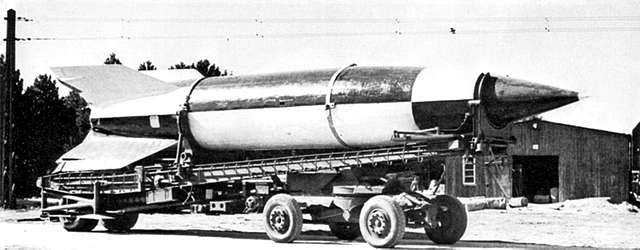
\includegraphics[width=0.75\linewidth]{figures/LiteratureStudy/V2_image.jpg}
    \caption{V2 rocket on Meillerwagen.\footnote{\url{https://timelessmoon.getarchive.net/media/v-2-rocket-on-meillerwagen-9effc8} (Accessed: 22 May 2025)}}
    \label{fig:V2_rocket}
\end{figure}

During the subsonic regime, under Mach 0.8, the drag is independent of the Mach number as compressibility effects are minimal. The lift coefficient has an initial increase with Mach number before a decrease, with the magnitude of the change observed being greater at higher angles of attack as the circulation around the rocket increases.

For the transonic regime, between Mach 0.8 and 1.2, shock waves begin to form and propagate over the rocket's surface, causing \textit{drag divergence}. Resulting in a rapid rise in drag approaching maximum drag and lift at 1.2. Strong shock and boundary layer interactions cause unsteady flow inducing the coefficient's rise.

\begin{figure}[H]
    \centering
    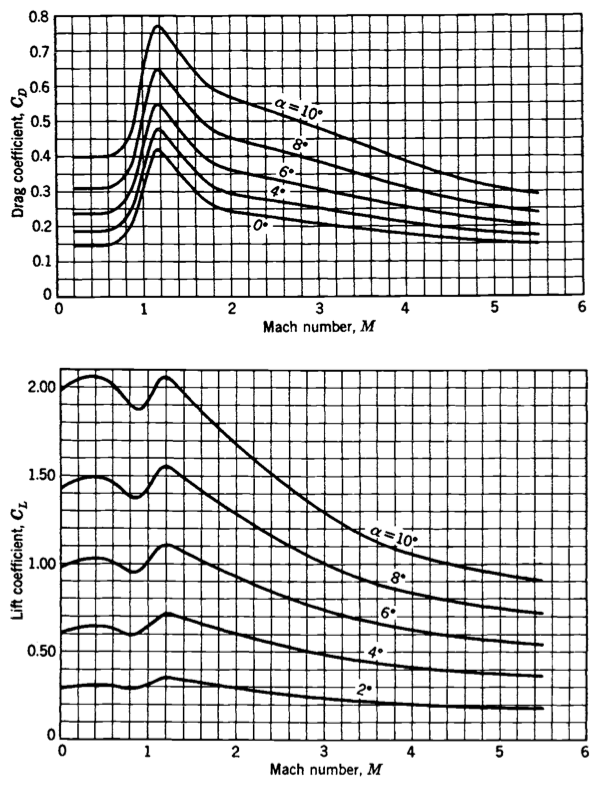
\includegraphics[width=0.75\linewidth]{figures/LiteratureStudy/V2-lift-drag-coefficient (1) (2).png}
    \caption{V2 rocket lift and drag coefficient curves (\cite{sutton_rocket_2016}).}
    \label{fig:V2_curves}
\end{figure}

The center of pressure (CoP) is the point on the rocket's body where the resultant aerodynamic force acts, in our case the lift and drag forces. \cite{TIR-33} states that a rocket during has aerodynamic stability if its center of pressure (CoP) is behind its center of gravity (CoG). A rocket may deviate for instance due to wind gusts, causing an increased angle of attack, a stable rocket will correct for this by forcing it back to zero over time. As a result, the center of pressure of the rocket is placed such that the rocket is aerodynamically stable during ascent and descent. A higher fidelity model for the center of pressure is not considered, as data on the V2 missile's center of pressure change with angle of attack and Mach number was not found. So the chosen CoP model cannot be validated, a constant center of pressure is taken.

The lift and drag coefficients of \autoref{fig:V2_curves} are converted to forces, lift and drag, through \autoref{eq:lift_drag}. Where the area $S$ is the cross-sectional area of the rocket, so $S = \pi \cdot r_r^2$, and the dynamic pressure is $q = \frac{1}{2} \cdot \rho \cdot V^2$.

\begin{equation}
\begin{aligned}
    L =& \frac{1}{2} \cdot \rho \cdot V^2 \cdot C_L \cdot S \\
    D =& \frac{1}{2} \cdot \rho \cdot V^2 \cdot C_D \cdot S
\end{aligned}
\label{eq:lift_drag}
\end{equation}

For the ascent phase, the center of pressure is behind the center of gravity, this gives the freebody diagram \autoref{fig:aero_reference_frames}, with angle of attack $\alpha$ the difference between the pitch and the flight path angle. Here two frames are present $(x',y')$ which is the initial reference frame, which is launchpad reference frame; x horizontal and right upward, translated to act at the rocket's center of gravity.$(x'',y'')$ is the body frame. From this freebody diagram the equations of motion can be derived, \autoref{eq:aero_forces_ascent}.

\begin{equation}
\begin{aligned}
    F_{x''} =& -L \cdot \cos(\alpha) -D\cdot\sin(\alpha) \\
    F_{y''} =& L \cdot \sin(\alpha) - D \cdot \cos(\alpha) \\
    M_z =& (d_{cg} - d_{cp}) \cdot ( -L \cdot \cos(\alpha) -D\cdot\sin(\alpha))
\end{aligned}
\label{eq:aero_forces_ascent}
\end{equation}

The center of pressure location is checked to find it's stable position with respect to the center of gravity. When an angle of attack is formed a negative aerodynamic moment is desired to correct the angle of attack. \autoref{eq:stability_ascent} derives the moments derivative with respect to angle of attack, before applying the small angle approximation. With a small $\alpha$ then $L\cdot \alpha << D$, and with the rest of the factors positive, the moment is restored.

\begin{equation}
\begin{aligned}
    \frac{dM_z}{d\alpha} =& (d_{cp} - d_{cg}) \cdot (L \cdot \sin(\alpha) -D \cdot \cos(\alpha) - C_{L_\alpha} q \cdot S\cdot \cos(\alpha) - C_{D_\alpha} \cdot q \cdot S \sin(\alpha)) \\
    =& (d_{cp} - d_{cg}) \cdot (L \cdot \alpha - D - C_{L_\alpha}\cdot q \cdot S - C_{D_\alpha} \cdot q \cdot S \cdot \alpha)
\end{aligned}
\label{eq:stability_ascent}
\end{equation}

The descent reference from of \autoref{fig:aero_reference_frames} is used to derive the body frame forces from the aerodynamics in \autoref{eq:descent_aero}. The effective angle of attack denotes the descent angle of attack which is found using \autoref{eq:eff_alpha}.

\begin{equation}
    \alpha_{eff} = \gamma - (\theta + \pi)
\label{eq:eff_alpha}
\end{equation}
        
\begin{equation}
\begin{aligned}
    F_{x''} =& -D \cdot \sin(\alpha_{eff}) - L \cdot \cos(\alpha_{eff}) \\
    F_{y''} =& D \cdot \cos(\alpha_{eff}) - L \cdot \sin(\alpha_{eff}) \\
     M_z =& (d_{cg} - d_{cp}) \cdot( -D \cdot \sin(\alpha_{eff}) - L \cdot \cos(\alpha_{eff}))
\end{aligned}
\label{eq:descent_aero}
\end{equation}

With the center of pressure now moved to the top of the rocket, the aerodynamic stability is checked in \autoref{eq:stability_descent}. For aerodynamic stability a positive restoring moment is required to minimise the angle of a. \autoref{eq:stability_descent} derives the moment derivative with respect to effective angle of attack before the small angle approximation is applied. A small angle of will make $L \cdot \alpha_{eff} << D$ so the applied moment is positive, as the rest of the terms are positive.

\begin{equation}
\begin{aligned}
    \frac{dM_z}{d\alpha_{eff}} =& (d_{cp} - d_{cg}) \cdot (C_{D_{\alpha_{eff}}} \cdot q \cdot S \cdot \sin(\alpha_{eff}) + C_{L_{\alpha_{eff}}} \cdot q \cdot S \cdot \cos(\alpha_{eff}) + D \cdot \cos(\alpha_{eff}) - L \cdot \sin(\alpha_{eff})) \\
    =& (d_{cp} - d_{cp}) \cdot (C_{D_{\alpha_{eff}}} \cdot q \cdot S \cdot \alpha_{eff} + C_{L_{\alpha_{eff}}} \cdot q \cdot S + D - L \cdot \alpha_{eff})
\end{aligned}
\label{eq:stability_descent}
\end{equation}

The translate into the inertia frame the transformations of \autoref{eq:inertial_aero} are performed, for descent and ascent.

\begin{equation}
\begin{aligned}
    F_{x'} =& F_{y''} \cdot \cos(\theta) + F_{x''} \cdot \sin(\theta) \\
    F_{y'} =& F_{y''} \cdot \sin(\theta) - F_{x''} \cdot \cos(\theta)
\end{aligned}
\label{eq:inertial_aero}
\end{equation}    

\begin{figure}[H]
    \centering
    \begin{subcaptionbox}{Ascent.}[0.45\linewidth]
        {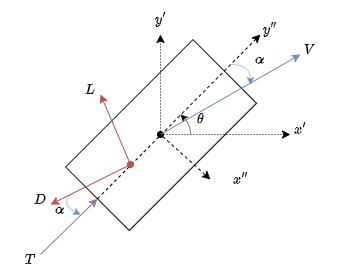
\includegraphics[width=\linewidth]{figures/LiteratureStudy/AerodynamicReference_ascent.png}}
        \label{fig:ascent_aero}
    \end{subcaptionbox}
    \hfill
    \begin{subcaptionbox}{Descent.}[0.45\linewidth]
        {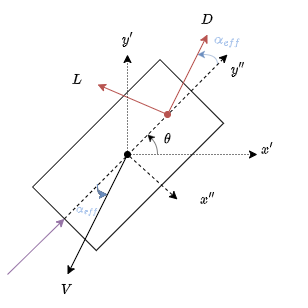
\includegraphics[width=\linewidth]{figures/LiteratureStudy/AerodynamicReference_descent (1).png} (1).png}
        \label{fig:descent_aero}
    \end{subcaptionbox}
    \caption{Aerodynamic Reference frames}
    \label{fig:aero_reference_frames}
\end{figure}

\subsection{Aerodynamic control surfaces}
\label{sec:ACS}
The aerodynamic control surfaces present on the rocket were chosen to grid fins in \autoref{sec:GNC}, as used on Space X's \textit{Super Heavy Booster}. Grid fins provide longitudinal and angular control, while also giving some drag to slow down the rocket. For Space X's electric motors torque the grid fins to their desired angle, as a result a first order low-pass filter can be used to model the lag in their actuation.

\cite{washington1993grid} perform experiments on grid fins and give curves for their drag and normal force coefficients, as these are validated examples of the change in aerodynamic coefficients for grid fins these shall be used as they provide a representative benchmark. The drag coefficient is roughly equal to the axial force coefficient of the grid fins at low angles of attack, as such \autoref{fig:drag_coeff_grid} can be interpolated by using \textit{WebPlotDigitiser} to extract points on the curve before linear interpolation. Washington also gives a curve for a curve for the change in the normal force coefficient with local angle of attack, \autoref{fig:cnalpha_grid}.

\begin{figure}[H]
    \centering
    \begin{subfigure}[b]{0.48\linewidth}
        \centering
        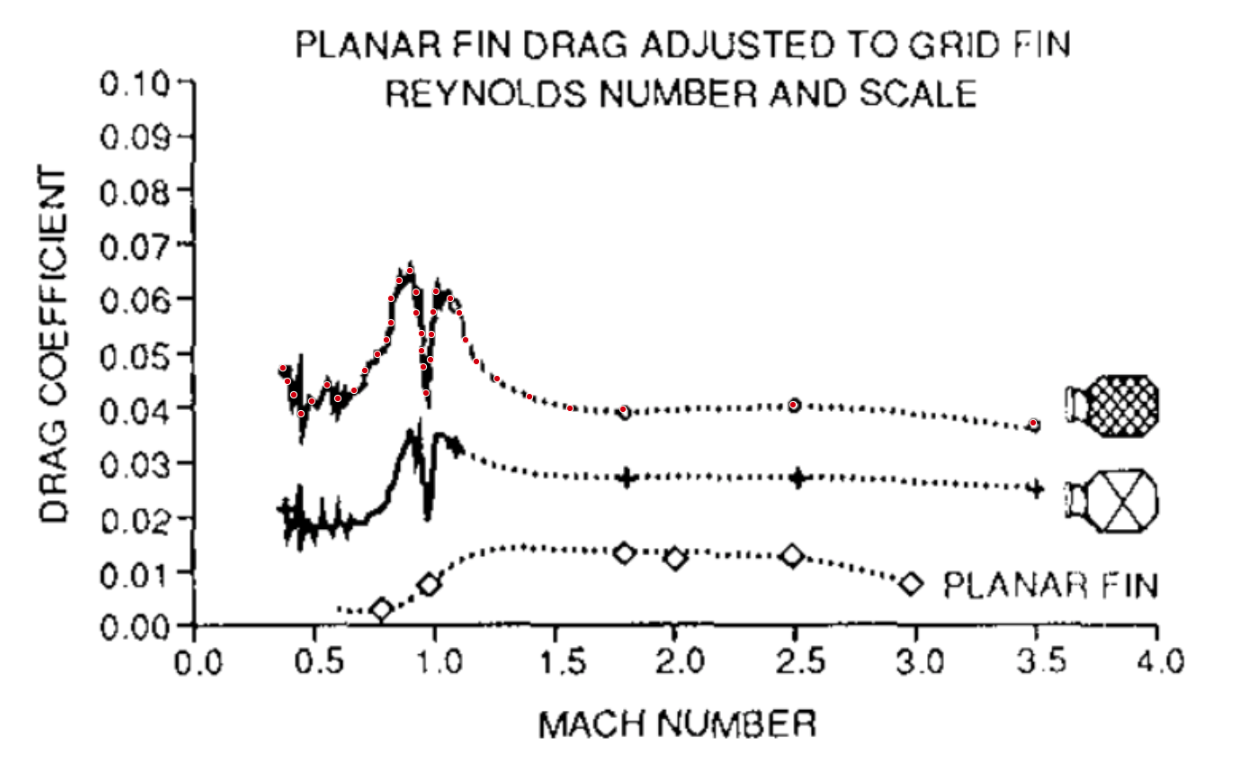
\includegraphics[width=\linewidth]{figures/LiteratureStudy/GridFins/DragCoefficientInterpolation.png}
        \caption{$C_D$ of a fin with points selected for interpolation \cite{washington1993grid}}
        \label{fig:drag_coeff_grid}
    \end{subfigure}
    \hfill
    \begin{subfigure}[b]{0.48\linewidth}
        \centering
        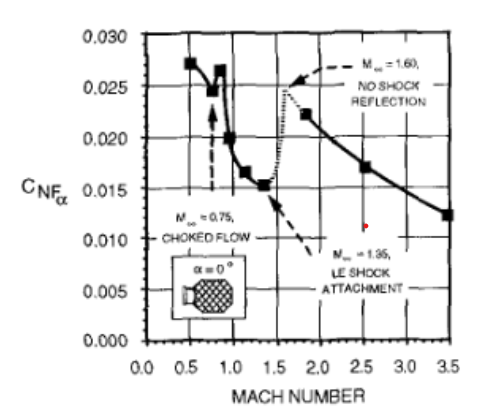
\includegraphics[width=\linewidth]{figures/LiteratureStudy/GridFins/CNGalpha_GF.png}
        \caption{$C_{N_\alpha}$ of a grid fin \cite{washington1993grid}}
        \label{fig:cnalpha_grid}
    \end{subfigure}
    \caption{Side-by-side comparison of drag coefficient and normal-force gradient for a grid fin}
    \label{fig:gridfin_side_by_side}
\end{figure}

The local angle of attack is the angle of the grid fin to the perpendicular direction of the flow. \autoref{eq:grid_fin_local_alpha} shows the local angle of attack for the left and right grid fins dependent on the effective angle of attack (descent angle of attack) and their respective deflection angles. The deflection angles go counter-clockwise, so an upward right grid fin deflection and a negative left grid fin deflection are positive.

\begin{equation}
\begin{aligned}
    \alpha_{l,R} =& \alpha_{eff} - \delta \\
    \alpha_{l,L} =& \alpha_{eff} + \delta 
\end{aligned}
\label{eq:grid_fin_local_alpha}
\end{equation}

With the angle of attack acting on each grid fin defined, the normal and axial force can be found from \autoref{fig:ACS_FBD}. First, the axial forces are the same for each grid fin as they are only dependent on Mach number. Second, the grid fins in the center of our 2D rocket are only modelled to give axial force as the third dimension is not considered.

\begin{equation}
\begin{aligned}
    F_a =& q \cdot S \cdot C_a(M) \\
    F_{N,L} =& q \cdot S \cdot C_n(M,\alpha_{l,L}) \\
    F_{N,R} =& q \cdot S \cdot C_n(M,\alpha_{l,R}) \\
\end{aligned}
\label{eq:grid_fin_aero_forces}
\end{equation}

The freebody diagram of the rocket during descent with grid fins is shown in \autoref{fig:ACS_FBD}. From this the perpendicular and parallel (x'', y'') forces are derived in \autoref{eq:ACS_para_perp}.

\begin{figure}[H]
    \centering
    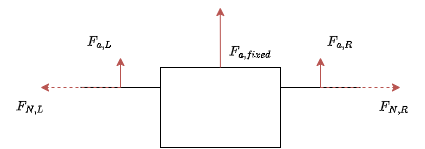
\includegraphics[width=0.5\linewidth]{figures/LiteratureStudy/GridFins/ACS_simple.png}
    \caption{Aerodynamic Control Surfaces freebody diagram during descent.}
    \label{fig:ACS_FBD}
\end{figure}

\begin{equation}
\begin{aligned}
    F_{x''} =& F_a \cdot (\cos(\delta_R) - \cos(\delta_L)) -F_{N,L} \cdot \cos(\delta_L) + F_{N_R} \cdot \cos(\delta_R) \\
    F_{y''} =& F_a \cdot (2 + \sin(\delta_L) + \sin(\delta_R)) - F_{N,L} \cdot \cos(\delta_L) + F_{N,R} \cdot \cos(\delta_R) \\
    M_z =& -(d_{gf}-d_{cg}) \cdot \bigg(F_a \cdot (\cos(\delta_R) - \cos(\delta_L)) -F_{N,L} \cdot \cos(\delta_L) + F_{N_R} \cdot \cos(\delta_R)\bigg) \\&+ r_r \cdot \bigg(F_{a} \cdot(\sin(\delta_R)-\sin(\delta_L) )+ F_{N,R} \cdot \cos(\delta_R) + F_{N,L} \cdot \cos(\delta_L)\bigg)
\end{aligned}
\label{eq:ACS_para_perp}
\end{equation}



\subsection{Atmosphere}
\label{sec:Atmosphere}
% ISA
% Gravity

Atmosphere dynamics influence the trajectory of the rocket, and the as such the control system design. Robust control systems need to adapt to disturbances and uncertainties, for instance wind in our case causing changes in relative velocities. Turbulence models, gusts, are often in the form of Dryden and von Karman models.

\cite{Mulder2020} state that the von Karman spectral densities are not rational functions, as such the Dryden model was introduced. However, the von Karman form does align better with experimental data, the Dryden form generally causes similar aircraft responses, as such the Dryden models shall be used.

Variations in relative velocity, caused by wind gusts, introduce dynamic changes that the control system must counteract in real time. Modelling these variations ensures a robust control strategy can be created to withstand them

As for atmosphere models, the International Standard Atmosphere (ISA) model is taken from \cite{Anderson2020Introduction}, and gravitational acceleration is calculated using \autoref{eq:grav}.

\begin{equation}
    g = g_0 \cdot \bigg(\frac{R_{E}}{R_{E} + y}\bigg)^2
\label{eq:grav}
\end{equation}


\subsection{Rocket engines}
\label{sec:RocketEngines}
The rocket engines provide the main source of acceleration to the rocket. Each engine/thruster is assumed to have identical throttle, and the gimballed thrusters identical gimbal angles, as explained in \autoref{sec:GNC} to limit the size of the action space for this benchmark study. To improve the simulation fidelity pressure losses have been included through \autoref{eq:pressure_losses}, because as the rocket moves through the atmosphere the atmospheric pressure will change altering the true thrust the thrusters enact on the rocket.

As the rocket burns propellant, fuel and oxidiser, will be consumed changing the mass of the rocket with the mass flow linearly scaled with throttle. Furthermore, a minimum of 40\% throttle per thruster has been enacted to keep inline with available thrusters. However, during descent the number of rocket engines active will decrease, this switching isn't modelled, but the central three thruster's are assumed always active as seen with the Super Heavy booster.

% Gimballing
The gimbal angle is defined as counter-clockwise to keep conventions uniform, this gives the body frame force's from the thrusters in \autoref{eq:thrust_ref}, with \autoref{eq:inertial_aero} providing the inertial frame translation.

\begin{equation}
\begin{aligned}
    F_{x''} =& - T^g \cdot \sin(\theta^g) \\
    F_{y''} =& T^{ng} + T^g \cdot \cos(\theta^g) \\
    M_z =& -(d_{cg} - d_{t}) T^g \cdot \sin(\theta^g)
\end{aligned}
\label{eq:thrust_ref}
\end{equation}

\subsection{Equations of motion}
\label{sec:EoM}
The previous subsections of this section has sized the rocket, and enacted forces upon the rocket. Here these will be collated together to form equations of motion for the rocket. The forces applied to the rocket are the some of the enacting forces in their respective axes. These forces come from the ACS, aerodynamics, thrusters and gravity, also apply moments to the body asides from gravity, with the RCS's cold gas thrusters applying a pure moment aswell when activated.

Newton's 2nd law, \autoref{eq:Netwons2nd}, converts the forces into the rocket's acceleration. The explicit first-order forward Euler numerical integration scheme is used to integrate acceleration into velocity and then position, as it offers a computationally inexpensive and easy to implement approach adequate for a low-fidelity simulation with a small time constant of 0.1 seconds.

\begin{equation}
    F= m \cdot a \rightarrow \ddot{x} = a = \frac{F}{m}
\label{eq:Netwons2nd}
\end{equation}

Euler's rotational motion equation, \autoref{eq:Euler_rotational}, is used to enact the moment's change on the orientation (pitch) of the rocket. The inertia changes and is updated as fuel is consumed, the model for derived for this inertia change is shown in \autoref{sec:inertia}. Again a explicit first-order forward Euler numerical integrations scheme is used.

\begin{equation}
    \ddot{\theta} = \frac{M}{I}
\label{eq:Euler_rotational}
\end{equation}